%\UseRawInputEncoding
\documentclass{article}
\setcounter{secnumdepth}{0}
\usepackage[T1]{fontenc}
\usepackage[utf8]{inputenc}
%\usepackage[latin1]{inputenc}
%\usepackage[english, norsk]{babel}
\usepackage{filecontents}
\usepackage{tcolorbox}
\usepackage{url}
\usepackage{etoolbox}
\usepackage{framed}
\usepackage{framed, color}
\usepackage{xcolor}
\usepackage{mdframed}
\usepackage{float}
\usepackage{gensymb}
\usepackage{amsmath}

\usepackage{caption}
\usepackage{subcaption}
\definecolor{Black}{rgb}{0.0, 0.0, 0.0}

%Definer kode
\usepackage{listings}
\usepackage{color}
\definecolor{dkgreen}{rgb}{0,0.6,0}
\definecolor{gray}{rgb}{0.5,0.5,0.5}
\definecolor{mauve}{rgb}{0.58,0,0.82}

\lstset{frame=tb,
extendedchars = true,
texcl=true,
  language=ADA,
  aboveskip=3mm,
  belowskip=3mm,
  showstringspaces=false,
  columns=flexible,
  basicstyle={\small\ttfamily},
  numbers=none,
  numberstyle=\tiny\color{gray},
  keywordstyle=\color{blue},
  commentstyle=\color{dkgreen},
  stringstyle=\color{mauve},
  breaklines=true,
  breakatwhitespace=true,
  tabsize=3
}

\usepackage[colorlinks]{hyperref}
\hypersetup{citecolor=Black}
\hypersetup{linkcolor=Black}
\hypersetup{urlcolor=Black}
\usepackage{cleveref}


\setlength{\parindent}{0em}
\setlength{\parskip}{1em}
%\renewcommand{\baselinestretch}{2.0}

%\renewcommand\thesubsection{\alph{subsection}}

\renewcommand{\figurename}{Figure}
\begin{document}
\author{Kent Odde}
\title{DDV3101 \\Cache Controller}

\maketitle
\thispagestyle{empty}
\begin{center}
\includegraphics[width=\linewidth,height=0.2\textheight,keepaspectratio]{img/USN.png}
\end{center}
\newpage

\tableofcontents

\newpage

\section{Abstract}

This is my submission for the semester project in DDV3101, fall 2020.

%Innholdsfortegnelse
\section{Introduction}
A cache controller is what administrates the cache memory. This assignment consists of implementing the cache controller design which is specified on page 462, in \textit{Computer organization \& Design: The Hardware/Software Interface}\cite{BOOK}

%Oppgaven
\section{Specifications}

The details of the design will become clear throughout the \textit{Implementation} section, however the key specifications for the cache controller design is as follows:
\begin{itemize}
  \item{Direct mapped}
  \item{Writeback using write allocate}
  \item{Block size: 4 words}
  \item{Cache size 16 KiB}
  \item{32-byte addresses}
\end{itemize}

A direct mapped cache controller means that in order to find the cache address for a memory address, we use this formula:

\begin{equation*}
  CacheAddress = (MemoryAddress) \bmod (Number\_of\_blocks\_in\_cache)
\end{equation*}

In other words, all the memory addresses which end in the same bits, will be mapped to the same cache address. This reduces overhead and lets us avoid expensive memory translation schemes. In order to know which actual memory address we have in our cache currently, we check the most significant bits of the address, against the tag stored in the cache at the index we need.

The fact that our cache is using writeback, means that when the CPU wants to write something to memory, we only write it to the cache. The new values will not be written back to memory until another memory address needs to take the current occupants place in the cache. This is a more efficient approach than for instance write-through, where we write back to both the memory and the cache every single time.

The cache controller is designed as a finite state machine, which can be seen in figure \ref{FSB}


\begin{figure}[H]
 \centering
  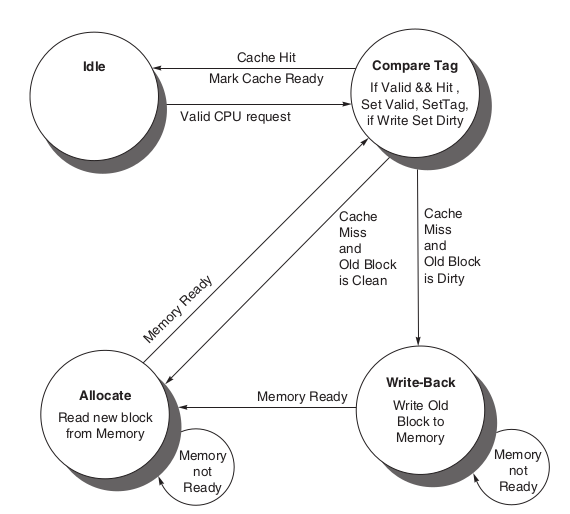
\includegraphics[width=300pt]{img/FSB.png}
  \caption{FSB\cite{BOOK}}
  \label{FSB}
 \end{figure}

An overview of the structure can be seen in figure \ref{OVERVIEW}.

\begin{figure}[H]
 \centering
  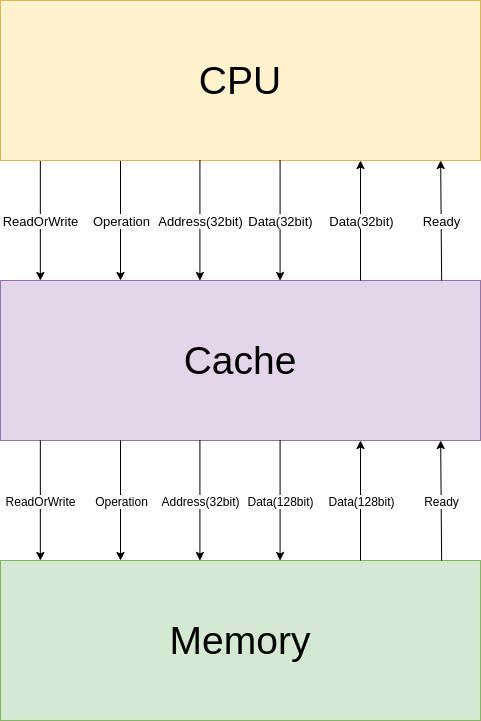
\includegraphics[width=300pt]{img/OverviewBlock.png}
 \caption{Overview}
  \label{OVERVIEW}
 \end{figure}

Lets have a look at how this will work. The CPU will send a 32 bit address to the cache. The cache will go into the state \textit{compare tag}. If we have a cache hit, it will return the correct block over the 32 bit bus to the CPU, and return to its \textit{idle}. However, if we have a miss, it will set the ready bit towards the CPU to 0, and check whether or not the index is valid and dirty. If this is the case, it means that we have to write back data, before we can fetch new the requested memory block into the cache. After the write-back, or if the write-back was not necessary, we move into the \textit{allocate} state, where we request the requested block from memory. The memory will give us 4 blocks on the 128 bit bus between the cache and memory. When this operation is complete, we go back to the \textit{compare tag} state, from where it will naturally return to the \textit{idle} state.


%Implementation
\section{Implementation}
\subsection{Structure}
In order to implement this in VHDL, the cache and the memory will be separate blocks. The ram block will consist of an array to simulate the memory. The cache will consist of one array to store the tags, dirty bits and valid bits, and another array for storing the actual data.

The CPU in our case will be the testbench, which will request different memory addresses, in order to test all the different outcomes of a memory access.

The more detailed specifications, can be seen in figure \ref{DETAILED}.

\begin{figure}[H]
 \centering
  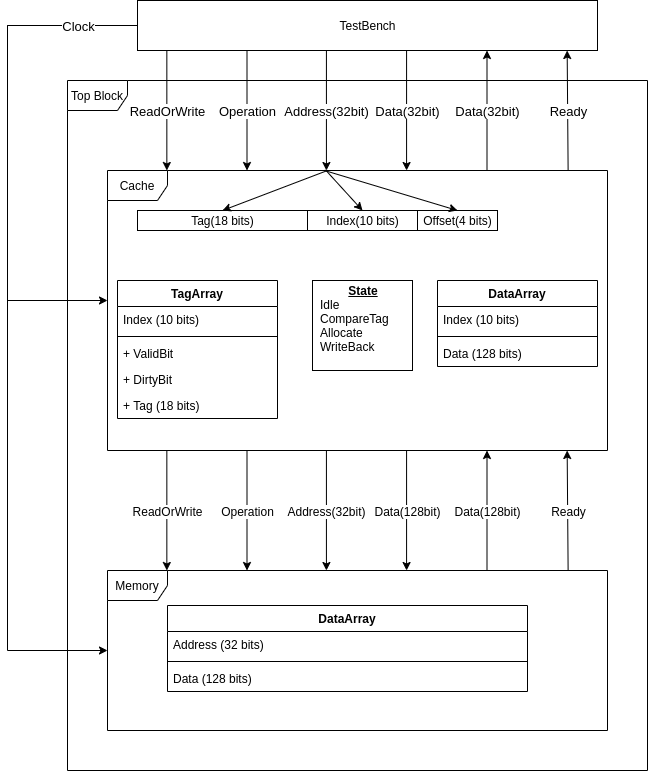
\includegraphics[width=300pt]{img/OverviewDetailed.png}
 \caption{Detailed structure}
  \label{DETAILED}
 \end{figure}

\subsection{The Code}

The source code can be seen in the appendices, and is commented quite richly.

The RAM and the top block is quite straightforward, however, the cache controller's FSB is quite a mess. The code was written before the professor's lecture on finite state machines, which means that the code is not structured as well as it should have been. However, since it took a thirteen hour debugging session to get it working, I really didn't want to try and refactor the code.

The top block has a lot of constants, which set the specifications, the plan was to write the code completely generic, so that a change in a constant variable, would change the specifications for the entire system. However, a lot of bugs within Vivado emerged when doing this on a large scale, and to get rid of the errors I had to hard-code a lot of the values throughout the program.

Because the address size is 32 bits, I tried implementing the memory as an array of 2**32 in size. However, as can be seen in figure \ref{ERROR}, this was not possible.
\begin{figure}[H]
 \centering
  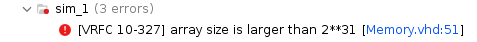
\includegraphics[width=300pt]{img/arraySizeError.png}
 \caption{Large array error}
  \label{ERROR}
 \end{figure}

Luckily it was possible to create arrays of 2**16, so that i would be able to at least circle around the cache once, and test for dirty misses.


\subsection{Schematic}
The generated schematic for the solution can be seen in figure \ref{SCHEMATIC}

\begin{figure}[H]
 \centering
  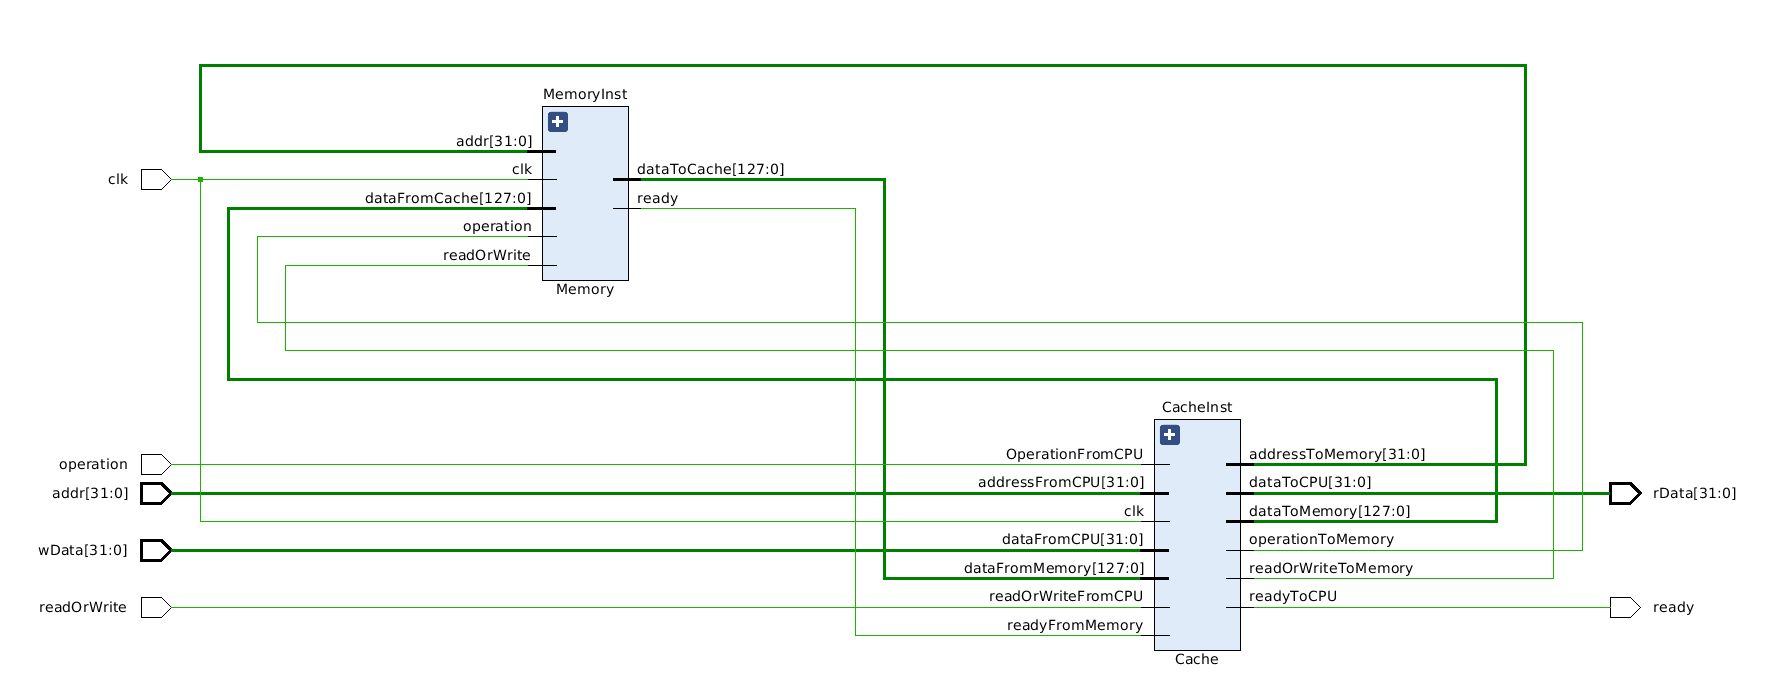
\includegraphics[width=400pt]{img/schematic211020.png}
 \caption{Schematic generated by Vivado}
  \label{SCHEMATIC}
 \end{figure}

Because of the scale of the implementation, this is the best schematic i can produce. Any attempt at trying opening the memory or cache in the elaboration design results in a software crash.

\subsection{Testbench}

In order to test all the cases, we need 8 operations from the CPU to the cache controller.

The eight operations consists of the following:
\begin{itemize}
  \item{Read from address 0, block 0. Should result in a miss}
  \item{Read from address 0, block 0. Should result in a hit}
  \item{Write to address 1, block 0. Should result in a miss}
  \item{Read from address 1, block 0. Should result in a hit}
  \item{Read from address 2, block 0. Should result in a miss}
  \item{Read from address 1024, block 0. Should result in a miss}
  \item{Read from address 1025, block 1. Should result in a \textbf{DIRTY} miss}
  \item{Write to address 1, block 1. Should result in a miss}
\end{itemize}

All of the data in the cache have been initialized to zeroes, and the data in RAM have been initialized to all ones in order to see what is going on.


In this initial state, we can see that the cache is completely empty
\begin{figure}[H]
\centering
\begin{subfigure}{.5\textwidth}
  \centering
  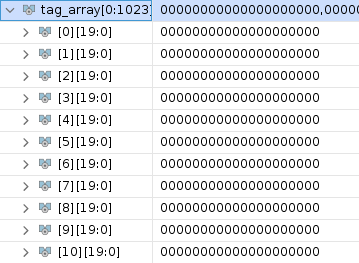
\includegraphics[width=.8\linewidth]{img/tag0.png}
  \caption{Tag array}
\end{subfigure}%
\begin{subfigure}{.5\textwidth}
  \centering
  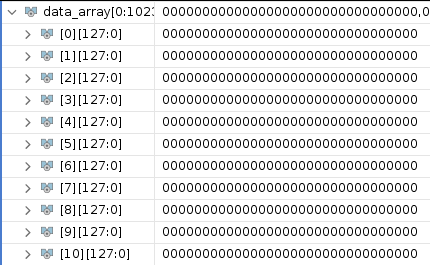
\includegraphics[width=.9\linewidth]{img/data0.png}
  \caption{Data array}
\end{subfigure}
\caption{Cache initial state}
\end{figure}


In the figure below, we have had our first operation, which inevitably was a miss, and we can see that index zero in the cache has been filled. The first bit in the tag-array is the valid bit.

The second operation is a hit on the same address, so it looks the exact same afterwards.
\begin{figure}[H]
\centering
\begin{subfigure}{.5\textwidth}
  \centering
  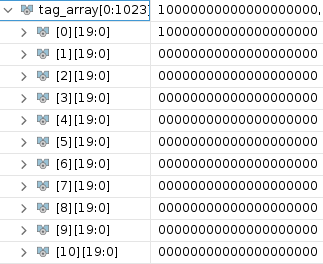
\includegraphics[width=.8\linewidth]{img/tag1.png}
  \caption{Tag array}
\end{subfigure}%
\begin{subfigure}{.5\textwidth}
  \centering
  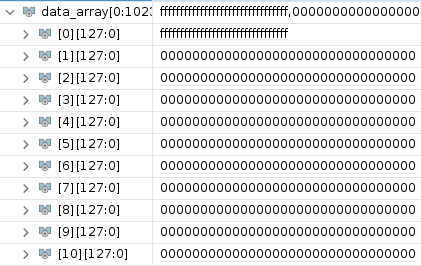
\includegraphics[width=.9\linewidth]{img/data1.png}
  \caption{Data array}
\end{subfigure}
\caption{After first operation}
\end{figure}





After the third operation, which was a clean write miss, we can see that index 1 in the cache has been read from memory, the first block has been written to, and the valid and dirty bit is active.

Since the fourth operation is a hit, the cache looks the same afterwards.
\begin{figure}[H]
\centering
\begin{subfigure}{.5\textwidth}
  \centering
  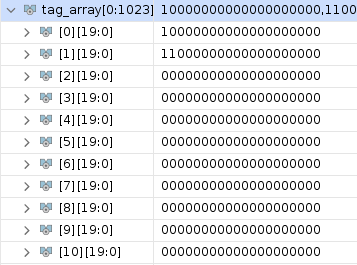
\includegraphics[width=.8\linewidth]{img/tag2.png}
  \caption{Tag array}
\end{subfigure}%
\begin{subfigure}{.5\textwidth}
  \centering
  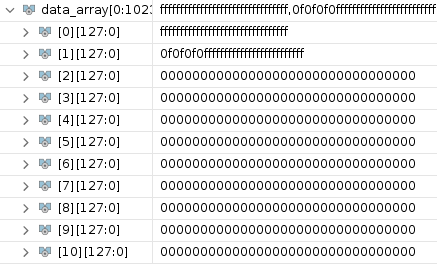
\includegraphics[width=.9\linewidth]{img/data2.png}
  \caption{Data array}
\end{subfigure}
\caption{Cache after third operation}
\end{figure}


The fifth operation is a read from address 2, block 0, which results in a miss. Index 2 has in the figure below been filled with the contents of the RAM at address 2.
\begin{figure}[H]
\centering
\begin{subfigure}{.5\textwidth}
  \centering
  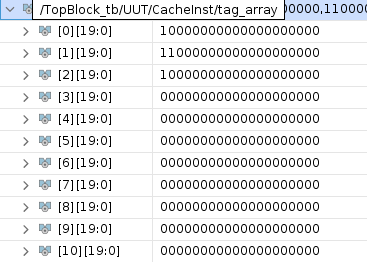
\includegraphics[width=.8\linewidth]{img/tag3.png}
  \caption{Tag array}
\end{subfigure}%
\begin{subfigure}{.5\textwidth}
  \centering
  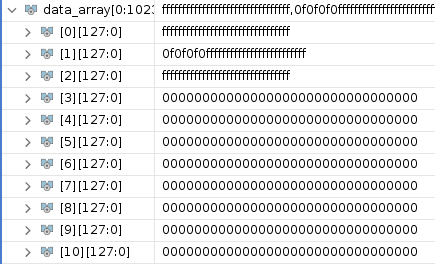
\includegraphics[width=.9\linewidth]{img/data3.png}
  \caption{Data array}
\end{subfigure}
\caption{After fifth operation}
\end{figure}


In the sixth operation we read from address 1024. This is a miss, which will throw out address 0 from the cache. In the tag-array, we can see that in index 0, the tags least significant bit is now higher than the others. Which is correct.
\begin{figure}[H]
\centering
\begin{subfigure}{.5\textwidth}
  \centering
  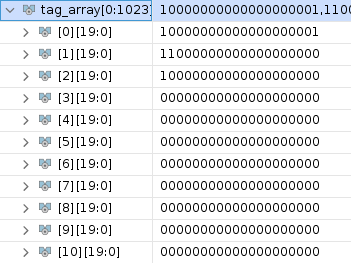
\includegraphics[width=.8\linewidth]{img/tag4.png}
  \caption{Tag array}
\end{subfigure}%
\begin{subfigure}{.5\textwidth}
  \centering
  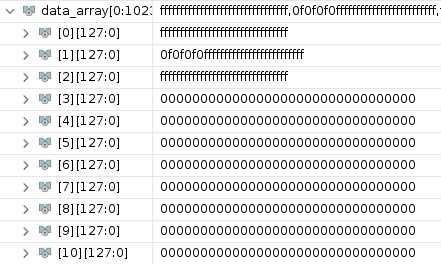
\includegraphics[width=.9\linewidth]{img/data4.png}
  \caption{Data array}
\end{subfigure}
\caption{After the sixth operation}
\end{figure}

The seventh operation, which is a dirty miss, will have to write back to memory before loading in from memory address 1025. In the figure below we can see how the contents of both the tag-array and data-array have changed at index 1.
\begin{figure}[H]
\centering
\begin{subfigure}{.5\textwidth}
  \centering
  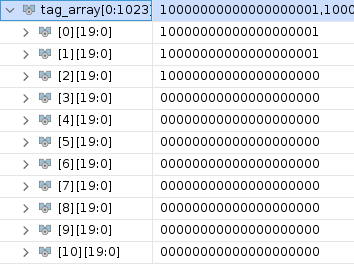
\includegraphics[width=.8\linewidth]{img/tag5.png}
  \caption{Tag array}
\end{subfigure}%
\begin{subfigure}{.5\textwidth}
  \centering
  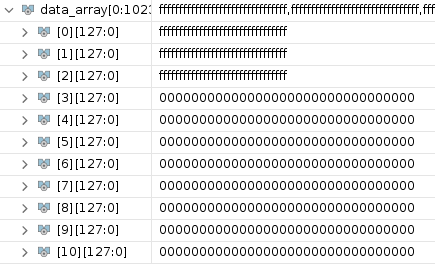
\includegraphics[width=.9\linewidth]{img/data5.png}
  \caption{Data array}
\end{subfigure}
\caption{After the seventh operation}
\end{figure}

Finally in the last operation, we write to address 1, block 1, which is a miss. As we already have written to address one, block 0, we can see the two first blocks of index 1 in the cache have different contents than the rest. We can also se the dirty and valid bit being active.
\begin{figure}[H]
\centering
\begin{subfigure}{.5\textwidth}
  \centering
  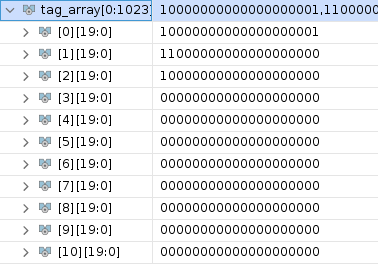
\includegraphics[width=.8\linewidth]{img/tag6.png}
  \caption{Tag array}
\end{subfigure}%
\begin{subfigure}{.5\textwidth}
  \centering
  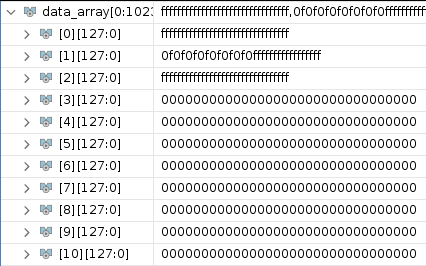
\includegraphics[width=.9\linewidth]{img/data6.png}
  \caption{Data array}
\end{subfigure}
\caption{After the eight operation}
\end{figure}


If we have a look at the testbench, we can se how the operations are much shorter on cache hits, then they are on misses:

\begin{figure}[H]
 \centering
  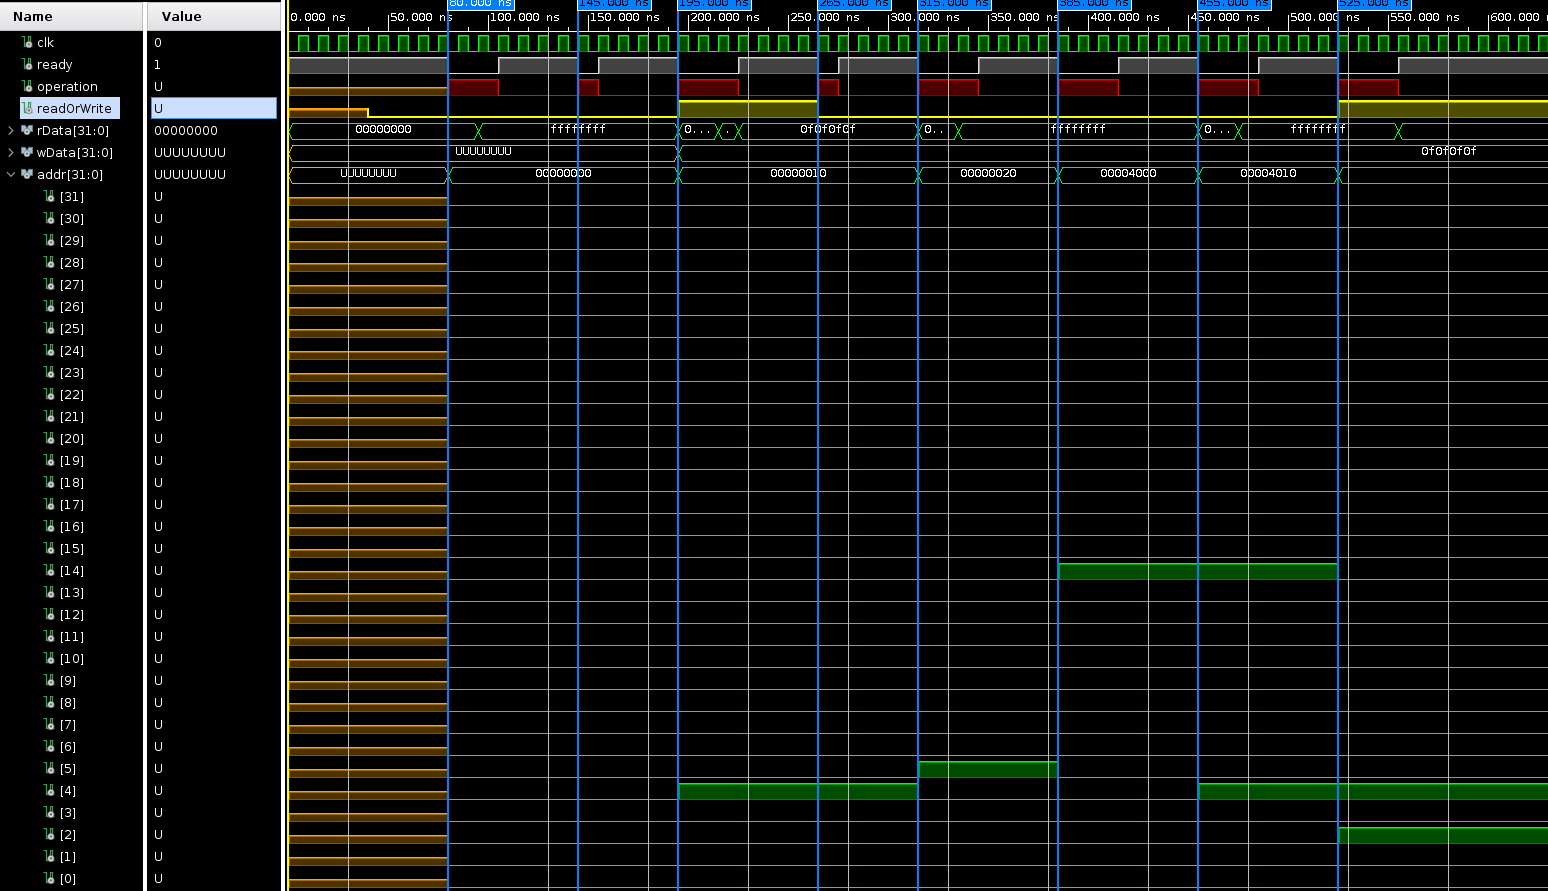
\includegraphics[width=400pt]{img/testbench1.png}
 \caption{Testbench}
  \label{TESTBENCH1}
 \end{figure}



%Konklusjon
\section{Conclusion}
This was a very fun, yet quite difficult exercise, with a high learning outcome. It took many readings of chapter 5 in the book, in order to understand caches well enough, and implementing the cache controller was very challenging. However, having done this I feel I have an understanding of cache memory, I wouldn't have had otherwise.

As mentioned, the code is by no means perfect, so please reach out to me if there is something unclear in the code or in this report.

%Vedlegg
\section{Appendices}
\subsection{Testbench}
\begin{lstlisting}
library IEEE;
use IEEE.STD_LOGIC_1164.ALL;

use IEEE.NUMERIC_STD.ALL;

entity TopBlock_tb is
--  Port ( );
end TopBlock_tb;

architecture Behavioral of TopBlock_tb is

    signal clk, ready, operation, readOrWrite : STD_LOGIC;
    signal rData, wData, addr : STD_LOGIC_VECTOR(31 downto 0);

    constant clk_period : time := 10 ns;
    --Define addressess for a more readable testbench
    --First digit refers to the address in decimal, and the second digit means which block we want
    signal address0_0 : std_logic_vector(31 downto 0) := std_logic_vector(to_unsigned(0, 28)) & "0000";
    signal address1_0 : std_logic_vector(31 downto 0) := std_logic_vector(to_unsigned(1, 28)) & "0000";
    signal address1_1 : std_logic_vector(31 downto 0) := std_logic_vector(to_unsigned(1, 28)) & "0100";
    signal address1_2 : std_logic_vector(31 downto 0) := std_logic_vector(to_unsigned(1, 28)) & "1000";
    signal address1_3 : std_logic_vector(31 downto 0) := std_logic_vector(to_unsigned(1, 28)) & "1100";
    signal address2_0 : std_logic_vector(31 downto 0) := std_logic_vector(to_unsigned(2, 28)) & "0000";
    signal address3_0 : std_logic_vector(31 downto 0) := std_logic_vector(to_unsigned(3, 28)) & "0000";
    signal address4_0 : std_logic_vector(31 downto 0) := std_logic_vector(to_unsigned(4, 28)) & "0000";
    signal address5_0 : std_logic_vector(31 downto 0) := std_logic_vector(to_unsigned(5, 28)) & "0000";

    signal address1024_0 : std_logic_vector(31 downto 0) := std_logic_vector(to_unsigned(1024, 28)) & "0000";
    signal address1025_0 : std_logic_vector(31 downto 0) := std_logic_vector(to_unsigned(1025, 28)) & "0000";
    signal address1025_1 : std_logic_vector(31 downto 0) := std_logic_vector(to_unsigned(1025, 28)) & "0100";
    signal address1025_2 : std_logic_vector(31 downto 0) := std_logic_vector(to_unsigned(1025, 28)) & "1000";
    signal address1025_3 : std_logic_vector(31 downto 0) := std_logic_vector(to_unsigned(1025, 28)) & "1100";
    signal address1026_0 : std_logic_vector(31 downto 0) := std_logic_vector(to_unsigned(1026, 28)) & "0000";
    signal address1027_0 : std_logic_vector(31 downto 0) := std_logic_vector(to_unsigned(1027, 28)) & "0000";
    signal address1028_0 : std_logic_vector(31 downto 0) := std_logic_vector(to_unsigned(1028, 28)) & "0000";
    signal address1029_0 : std_logic_vector(31 downto 0) := std_logic_vector(to_unsigned(1029, 28)) & "0000";

    constant writeData : std_logic_vector(31 downto 0) := "00001111000011110000111100001111";

    component TopBlock is
    Port (  clk :       in STD_LOGIC := '1';
            ready : out STD_LOGIC := '1';
            operation : in STD_LOGIC := '0';
            rData :     out STD_LOGIC_VECTOR (31 downto 0) := (others => '0');--(Word-1 downto 0);
            addr :      in STD_LOGIC_VECTOR (31 downto 0):= (others => '0');--(AddressBits-1 downto 0);
            wData :     in STD_LOGIC_VECTOR (31 downto 0):= (others => '0');--(Word-1 downto 0);
            readOrWrite :      in STD_LOGIC);
end component TopBlock;



begin
    UUT: TopBlock
    Port Map(    clk => clk, ready => ready, operation => operation, readOrWrite => readOrWrite,
                rData => rData, wData => wData, addr => addr);


    clk_process : process
    begin
        clk <= '0';
        wait for clk_period/2;
        clk <= '1';
        wait for clk_period/2;
    end process;


    stim_proc : process
    begin
    --Read from addr0: MISS,
        wait for clk_period*4;
        readOrWrite <= '0';

        wait for clk_period*4;
        addr <= address0_0;
        readOrWrite <= '0';
        operation <= '1';
        wait until ready = '1';
        operation <= '0';

        wait for clk_period*4;

    --Read from addr0: HIT
        addr <= address0_0;
        readOrWrite <= '0';
        operation <= '1';
        wait until ready = '1';
        operation <= '0';

        wait for clk_period*4;

    --Write to addr1\_0: MISS, NOT DIRTY
        addr <= address1_0;
        wData <= writeData;

        readOrWrite <= '1';
        operation <= '1';
        wait until ready = '1';
        operation <= '0';

        wait for clk_period*4;

    --Read from addr1\_0: HIT
        addr <= address1_0;
        readOrWrite <= '0';
        operation <= '1';
        wait until ready = '1';
        operation <= '0';

        wait for clk_period*4;

    --read from addr2\_0: MISS
        addr <= address2_0;
        readOrWrite <= '0';
        operation <= '1';
        wait until ready = '1';
        operation <= '0';

        wait for clk_period*4;

    --read from addr1024\_0: CLEAN MISS
        addr <= address1024_0;
        readOrWrite <= '0';
        operation <= '1';
        wait until ready = '1';
        operation <= '0';

        wait for clk_period*4;

    --read from addr1025\_0: DIRTY MISS
        addr <= address1025_0;
        readOrWrite <= '0';
        operation <= '1';
        wait until ready = '1';
        operation <= '0';

        wait for clk_period*4;


    --Write to addr1\_1: MISS, NOT DIRTY
        addr <= address1_1;
        wData <= writeData;
        readOrWrite <= '1';
        operation <= '1';
        wait until ready = '1';
        operation <= '0';

        wait for clk_period*4;

        wait;
    end process;

end Behavioral;
\end{lstlisting}
\subsection{Top-Block}
\begin{lstlisting}
library IEEE;
use IEEE.STD_LOGIC_1164.ALL;
use IEEE.Math_real.all;

entity TopBlock is
    Port (  clk :       in STD_LOGIC := '1';
            ready : out STD_LOGIC := '1';
            operation : in STD_LOGIC := '0';
            rData :     out STD_LOGIC_VECTOR (31 downto 0) := (others => '0');
            addr :      in STD_LOGIC_VECTOR (31 downto 0):= (others => '0');
            wData :     in STD_LOGIC_VECTOR (31 downto 0):= (others => '0');
            readOrWrite :      in STD_LOGIC);
end TopBlock;

architecture Behavioral of TopBlock is
    --Constants
    constant Byte : Integer := 8; --(2**3)
    constant Kibi : Integer := 1024; --(2**10)
    constant Word : Integer := 32; --(2**5)
    constant BlockSize : Integer := 4 * Word; --128 (2**7)
    constant CacheSizeBits : Integer := 16 * Kibi * Byte; --16KiB
    constant CacheBlockSize : Integer := CacheSizeBits / BlockSize; --1024 (2**10)
    constant AddressBits : Integer := 32; --32 Bytes
    constant ValidBitSize : Integer := 1;
    constant DirtyBitSize : Integer := 1;
    constant N : Integer := Integer(log2(Real(CacheBlockSize))); --10
    constant M : Integer := Integer(log2(Real(BlockSize/Word))); -- 2

    constant indexSize : Integer := N; -- 10
    constant tagSize : Integer := 18;--32 - (n + m + 2);  --18

    constant offsetSize : Integer := 4;

    --Output from cacheController
    signal cache2MemReadOrWrite : STD_LOGIC := '0';
    signal cache2MemAddress : STD_LOGIC_VECTOR(addressBits-1 downto 0) := (others => '0');
    signal cache2MemData : STD_LOGIC_VECTOR(BlockSize -1 downto 0) := (others => '0');
    signal cache2MemOperation : STD_LOGIC := '0';

    --Output from Memory
    signal mem2CacheReady : STD_LOGIC := '0';
    signal mem2CacheData : STD_LOGIC_VECTOR(BlockSize-1 downto 0) := (others => '0');

    --Components
    Component Memory
        Generic(    addressBits : Integer;
                    BlockSize : Integer);
        Port ( clk :            in STD_LOGIC;
               readOrWrite :    in STD_LOGIC;
               operation :      in STD_LOGIC;
               addr :           in STD_LOGIC_VECTOR (addressBits-1 downto 0);
               --Må være 128 bit:
               dataFromCache :  in STD_LOGIC_VECTOR (BlockSize-1 downto 0);
               dataToCache :    out STD_LOGIC_VECTOR (BlockSize-1 downto 0);
               ready : out STD_LOGIC);
    end Component Memory;

    Component Cache
        Generic(    addressBits : Integer;
                    BlockSize : Integer;
                    WordSize : Integer;
                    offsetSize : Integer;
                    indexSize : Integer;
                    tagSize : Integer);

        Port ( clk :                in STD_LOGIC;
               readOrWriteFromCPU : in STD_LOGIC;
               OperationFromCPU :   in STD_LOGIC;
               addressFromCPU :     in STD_LOGIC_VECTOR(addressBits-1 downto 0);
               dataToCPU :          out STD_LOGIC_VECTOR (Word-1 downto 0);
               dataFromCPU :        in STD_LOGIC_VECTOR (Word-1 downto 0);
               readyToCPU :         out STD_LOGIC;

               dataFromMemory :     in STD_LOGIC_VECTOR(BlockSize-1 downto 0);
               dataToMemory :       out STD_LOGIC_VECTOR(BlockSize-1 downto 0);
               addressToMemory :    out STD_LOGIC_VECTOR(addressBits-1 downto 0);
               operationToMemory :  out STD_LOGIC;
               readOrWriteToMemory: out STD_LOGIC := '0';
               readyFromMemory :    in STD_LOGIC);
    end Component Cache;

begin
    CacheInst : Cache
    Generic Map(addressBits => AddressBits, BlockSize => BlockSize, WordSize => Word, indexSize => indexSize, offsetSize => offsetSize, tagSize => tagSize)
    Port Map(   clk => clk,
                readOrWriteFromCPU => readOrWrite,
                operationFromCPU => operation,
                addressFromCPU => addr,
                dataToCPU => rData,
                dataFromCPU => wData,
                readyToCPU => ready,
                dataFromMemory => mem2CacheData,
                dataToMemory => cache2MemData,
                addressToMemory => cache2MemAddress,
                operationToMemory => cache2MemOperation,
                readOrWriteToMemory => cache2MemReadOrWrite,
                readyFromMemory => mem2CacheReady);

    MemoryInst : Memory
    Generic Map(addressBits => AddressBits, BlockSize => BlockSize)
    Port Map(   clk => clk,
                readOrWrite => cache2MemReadOrWrite,
                operation => cache2MemOperation,
                addr => cache2MemAddress,
                dataFromCache => cache2MemData,
                dataToCache => mem2CacheData,
                ready => mem2CacheReady);

end Behavioral;
\end{lstlisting}

\subsection{Cache Controller}
\begin{lstlisting}
library IEEE;
use IEEE.STD_LOGIC_1164.ALL;

use IEEE.NUMERIC_STD.ALL;

entity Cache is
    Generic(    addressBits : Integer;
                BlockSize : Integer;
                WordSize : Integer;
                offsetSize : Integer;
                indexSize : Integer;
                tagSize : Integer);

        Port ( clk :                in STD_LOGIC;
               readOrWriteFromCPU : in STD_LOGIC;
               OperationFromCPU :   in STD_LOGIC;
               addressFromCPU :     in STD_LOGIC_VECTOR(addressBits-1 downto 0);
               dataToCPU :          out STD_LOGIC_VECTOR (WordSize-1 downto 0);
               dataFromCPU :        in STD_LOGIC_VECTOR (WordSize-1 downto 0);
               readyToCPU :         out STD_LOGIC;

               --Disse må være 128 bit
               dataFromMemory :     in STD_LOGIC_VECTOR(BlockSize-1 downto 0);
               dataToMemory :       out STD_LOGIC_VECTOR(BlockSize-1 downto 0);
               addressToMemory :    out STD_LOGIC_VECTOR(addressBits-1 downto 0);
               operationToMemory :  out STD_LOGIC;
               readOrWriteToMemory: out STD_LOGIC := '0';
               readyFromMemory :      in STD_LOGIC);
end Cache;

architecture Behavioral of Cache is

    Component FourToOneMux
    Generic (BlockSize : Integer;
                WordSize : Integer);
    Port ( i0 : in STD_LOGIC_VECTOR (BlockSize-1 downto 0);
           sel : in STD_LOGIC_VECTOR (1 downto 0);
           Y : out STD_LOGIC_VECTOR (WordSize-1 downto 0));
    end Component FourToOneMux;

    constant ValidBitIndex : Integer := (tagSize - 1 + 2);
    constant DirtyBitIndex : Integer := tagSize - 1 + 1;

    --Parse input address:
    signal tag : STD_LOGIC_VECTOR(tagsize-1 downto 0) := (others => '0');
    signal index : STD_LOGIC_VECTOR(9 downto 0) := (others => '0');
    signal byteOffset : STD_LOGIC_VECTOR(1 downto 0) := (others => '0');

    type state_type is (Idle, CompareTag, Allocate, WriteBack);
    signal state : state_type := Idle;
    signal state_next : state_type := Idle;

    --ARRAY OF TAGS
    --VALID BIT, DIRTY BIT and the TAG (LSB);
    type tag_array_type is array(0 to (2**index'length)-1 ) of std_logic_vector(ValidBitIndex downto 0);
    signal tag_array : tag_array_type := (others => (others => '0'));

    --ARRAY OF DATA
    type memory_type is array(0 to 1023) of std_logic_vector(BlockSize-1 downto 0);
    signal data_array : memory_type := (others => (others => '0'));

    signal current_data : std_logic_vector(BlockSize-1 downto 0);
begin
    --Update all necessary stuff
    tag <= addressFromCPU(31 downto 14);
    index <= addressFromCPU(13 downto 4);
    byteOffset <= addressFromCPU(3 downto 2);
    current_data <= data_array(to_integer(unsigned(index)));

    --Setup mux for writing a word from CPU to cache
    Mux : FourToOneMux
    Generic Map(BlockSize => BlockSize, WordSize => WordSize)
    Port Map(i0 => current_data, sel => byteOffset, Y => dataToCPU);

    --State register part
    process(clk, addressFromCPU)
    begin
        if(rising_edge(clk)) then
            state <= state_next;
        end if;
    end process;

    -- Next state Logic
    process(state, index, tag, tag_array, operationFromCPU, addressFromCPU, dataFromCPU, dataFromMemory, readyFromMemory)
    begin
        case state is
            when Idle =>
                --Checks for an operation from CPU, if not stay in current state
                if (OperationFromCPU = '1') then
                    state_next <= compareTag;
                else
                    state_next <= state;
                end if;


            when CompareTag =>
                --If valid bit in index is equal to 1 (IE VALID) and TAG Matches:
                --HIT!!!
                if(tag_array(to_integer(unsigned(index)))(ValidBitIndex) = '1') and
                    (tag_array(to_integer(unsigned(index)))(tagSize-1 downto 0) = tag) then

                    --If its a hit, it does not matter whether its a read or write, we are going back either way
                    state_next <= idle;

                --MISS
                else
                    --If cache miss and old block is clean, goto allocate
                    if(tag_array(to_integer(unsigned(index)))(DirtyBitIndex) = '0') then
                        state_next <= Allocate;

                    --If dirty bit, we have to write back!!
                    else
                        state_next <= writeBack;
                    end if;
                end if;


            when Allocate =>
                --If Memory ready, return to compare tag
                if(readyFromMemory = '1') then
                    state_next <= CompareTag;

                --Memory not ready, keep waiting
                else
                    state_next <= state;
                end if;


            when WriteBack =>
                --If memory ready, goto to allocate
                if(readyFromMemory = '1') then
                    state_next <= Allocate;
                --If not ready, keep waiting
                else
                    state_next <= state;
                end if;
        end case;
    end process;


    --Output logic;
    process(state, state_next, readOrWriteFromCPU, OperationFromCPU, addressFromCPU, dataFromCPU, dataFromMemory, readyFromMemory, index, tag, byteOffset) is
    begin
        case state is
            when Idle =>
            --Let cpu know we are idle, and let memory know that there is no current operation.
                if(state_next = CompareTag) then
                    readyToCPU <= '0';
                else
                    operationToMemory <= '0';
                    readyToCPU <= '1';
                end if;

            when CompareTag =>
                if(state_next = idle) then
                    --Checking if we were writing
                    if(readOrWriteFromCPU = '1') then
                        --Set Dirty Bit, if we were writing
                        tag_array(to_integer(unsigned(index)))(DirtyBitIndex) <= '1';
                        --The book says that we also have to set the tag and valid bit, but this is due to some strange implementation i believe. In this solution I don't think this is necessary.

                        --Write the data from CPU into cache
                        case byteOffset is
                            when "00" =>
                                data_array(to_integer(unsigned(index)))(127 downto 96) <= dataFromCPU;
                            when "01" =>
                                data_array(to_integer(unsigned(index)))(95 downto 64) <= dataFromCPU;
                            when "10" =>
                                data_array(to_integer(unsigned(index)))(63 downto 32) <= dataFromCPU;
                            when others =>
                                data_array(to_integer(unsigned(index)))(31 downto 0) <= dataFromCPU;
                        end case;
                    end if;
                    --Tell the processor that we are ready if we are on our way back to idle.
                    readyToCPU <= '1';

                --If next state is allocate, we need to let the memory know what we need
                elsif(state_next = Allocate) then

                    addressToMemory <= addressFromCPU;
                    readOrWriteToMemory <= '0';
                    --Tell memory that an operation is underway:
                    operationToMemory <= '1';

                --If next state is writeBack, we need to give the memory the stuff it needs
                elsif(state_next = WriteBack) then
                    addressToMemory <= tag_array(to_integer(unsigned(index)))(17 downto 0) & index & "0000";
                    dataToMemory <= data_array(to_integer(unsigned(index)));
                    readOrWriteToMemory <= '1';
                    operationToMemory <= '1';
                    --We also have to set the dirtybit to 0, so that we can write to the cache location after the writeback and allocation
                    tag_array(to_integer(unsigned(index)))(DirtyBitIndex) <= '0';
                else
                    --Should never get here, but for some reason, sometimes we do.
                    null;
                end if;

            when Allocate =>
                if(readyFromMemory = '1') then
                    --When the memory has put the necessary data on the bus, we can read it, and store it in cache.
                    tag_array(to_integer(unsigned(index))) <= '1' & '0' & tag;
                    data_array(to_integer(unsigned(index))) <= dataFromMemory;
                end if;

            --Nothing to be outputed in this state.
            when WriteBack =>
                null;
        end case;
   end process;
end Behavioral;

\end{lstlisting}

\subsection{RAM}
\begin{lstlisting}
library IEEE;
use IEEE.STD_LOGIC_1164.ALL;

use IEEE.NUMERIC_STD.ALL;

entity Memory is
    Generic(    addressBits : Integer;
                BlockSize : Integer);
    Port ( clk :            in STD_LOGIC;
           readOrWrite :    in STD_LOGIC;
           operation :      in STD_LOGIC;
           addr :           in STD_LOGIC_VECTOR (31 downto 0);
           --Må være 128 bit:
           dataFromCache :  in STD_LOGIC_VECTOR (127 downto 0);
           dataToCache :    out STD_LOGIC_VECTOR (127 downto 0);
           ready : out STD_LOGIC);
end Memory;

architecture Behavioral of Memory is
    --Vivado won't let me have arrays of the intended size (2**32)-1.
    --This smaller array lets me at least use addresses of the first and second "modulodegree", so I have been able to test the cache.
    type memory_type is array(0 to (2**16)-1) of std_logic_vector(127 downto 0);
    signal RAM : memory_type := (others => (others => '1'));
begin
    process(clk, operation, readOrWrite, addr)
    begin
        if(operation = '1') then
            ready <= '0';
            case readOrWrite is
                when '0' =>
                    dataToCache <= RAM(to_integer(unsigned(addr(31 downto 4))));
                when others =>
                    RAM(to_integer(unsigned(addr(31 downto 4)))) <= dataFromCache;
            end case;
        end if;
        ready <= '1';
    end process;
end Behavioral;
\end{lstlisting}

\subsection{Mux}
\begin{lstlisting}
library IEEE;
use IEEE.STD_LOGIC_1164.ALL;

entity FourToOneMux is
    Generic (BlockSize : Integer;
                WordSize : Integer);
    Port ( i0 : in STD_LOGIC_VECTOR (BlockSize - 1 downto 0);
           sel : in STD_LOGIC_VECTOR (1 downto 0);
           Y : out STD_LOGIC_VECTOR (WordSize - 1 downto 0));
end FourToOneMux;

architecture Behavioral of FourToOneMux is

begin

    Y <=    i0(127 downto 96) when sel = "00" else
            i0(95 downto 64) when sel = "01" else
            i0(63 downto 32) when sel = "10" else
            i0(31 downto 0);
end Behavioral;
\end{lstlisting}
\newpage
%Referanse
%\section{Referanser}

\nocite{*}
\bibliographystyle{plain}
\bibliography{ref}

\addcontentsline{toc}{section}{References}

\end{document}
